% \VignetteIndexEntry{caret Manual -- Model Building}
% \VignetteDepends{caret}
% \VignettePackage{caret}
\documentclass[12pt]{article}
\usepackage{colortbl}
\usepackage{amsmath}
\usepackage[pdftex]{graphicx}
\usepackage{color}
\usepackage{xspace}
\usepackage{fancyvrb}
\usepackage{fancyhdr}
\usepackage{lastpage}
\usepackage{longtable} 
\usepackage[boxed, linesnumbered]{algorithm2e}
\usepackage[
         colorlinks=true,
         linkcolor=blue,
         citecolor=blue,
         urlcolor=blue]
         {hyperref}
\usepackage{lscape}

\usepackage{Sweave}

%%%%%%%%%%%%%%%%%%%%%%%%%%%%%%%%%%%%%%%%%%%%%%%%%%%%%%%%%%%%%%%%%%

% define new colors for use
\definecolor{darkgreen}{rgb}{0,0.6,0}
\definecolor{darkred}{rgb}{0.6,0.0,0}
\definecolor{lightbrown}{rgb}{1,0.9,0.8}
\definecolor{brown}{rgb}{0.6,0.3,0.3}
\definecolor{darkblue}{rgb}{0,0,0.8}
\definecolor{darkmagenta}{rgb}{0.5,0,0.5}

%%%%%%%%%%%%%%%%%%%%%%%%%%%%%%%%%%%%%%%%%%%%%%%%%%%%%%%%%%%%%%%%%%

\newcommand{\bld}[1]{\mbox{\boldmath $#1$}}
\newcommand{\shell}[1]{\mbox{$#1$}}
\renewcommand{\vec}[1]{\mbox{\bf {#1}}}

\newcommand{\code}[1]{\mbox{\footnotesize\color{darkblue}\texttt{#1}}}
\newcommand{\pkg}[1]{{\fontseries{b}\selectfont #1}}
\renewcommand{\pkg}[1]{{\textsf{#1}}}

\newcommand{\ReallySmallSpacing}{\renewcommand{\baselinestretch}{.6}\Large\normalsize}
\newcommand{\SmallSpacing}{\renewcommand{\baselinestretch}{1.1}\Large\normalsize}

\newcommand{\halfs}{\frac{1}{2}}

\setlength{\oddsidemargin}{-.25 truein}
\setlength{\evensidemargin}{0truein}
\setlength{\topmargin}{-0.2truein}
\setlength{\textwidth}{7 truein}
\setlength{\textheight}{8.5 truein}
\setlength{\parindent}{0truein}
\setlength{\parskip}{0.10truein}


\DefineVerbatimEnvironment{Sinput}{Verbatim}{fontshape=sl,formatcom=\color{darkblue}} 
\fvset{listparameters={\setlength{\topsep}{0pt}}}
\renewenvironment{Schunk}{\vspace{\topsep}}{\vspace{\topsep}}

\fvset{fontsize=\footnotesize}
 

%%%%%%%%%%%%%%%%%%%%%%%%%%%%%%%%%%%%%%%%%%%%%%%%%%%%%%%%%%%%%%%%%%
\pagestyle{fancy}
\lhead{}
\chead{The {\tt caret} Package}
\rhead{}
\lfoot{}
\cfoot{}
\rfoot{\thepage\ of \pageref{LastPage}}
\renewcommand{\headrulewidth}{1pt}
\renewcommand{\footrulewidth}{1pt}
%%%%%%%%%%%%%%%%%%%%%%%%%%%%%%%%%%%%%%%%%%%%%%%%%%%%%%%%%%%%%%%%%%

\title{The {\tt caret} Package}
\author{Max Kuhn \\ max.kuhn@pfizer.com}


\begin{document}

\maketitle
\renewcommand{\baselinestretch}{.6}

\tableofcontents

\thispagestyle{empty}
	
\vspace{.2in}

\renewcommand{\baselinestretch}{1}
 
	
	


The \pkg{caret} package (short for
{\bf{\color{blue}{c}}}lassification {\bf{\color{blue}{a}}}nd
{\bf{\color{blue}{re}}}gression {\bf{\color{blue}{t}}}raining)
contains functions to streamline the model training process for
complex regression and classification problems. The package utilizes a
number of R packages but tries not to load them all at package
start-up\footnote{By adding formal package dependencies, the package
  startup time can be greatly decreased}. The package ``suggests''
field includes: \pkg{ada}, \pkg{affy}, \pkg{Boruta}, \pkg{bst}, \pkg{caTools}, \pkg{class}, \pkg{Cubist}, \pkg{doMC}, \pkg{e1071}, \pkg{earth ($\ge$ 2.2-3)}, \pkg{elasticnet}, \pkg{ellipse}, \pkg{fastICA}, \pkg{foba}, \pkg{gam}, \pkg{GAMens ($\ge$ 1.1.1)}, \pkg{gbm}, \pkg{glmnet}, \pkg{gpls}, \pkg{grid}, \pkg{hda}, \pkg{HDclassif}, \pkg{Hmisc}, \pkg{ipred}, \pkg{kernlab}, \pkg{klaR}, \pkg{lars}, \pkg{leaps}, \pkg{LogicForest}, \pkg{logicFS}, \pkg{LogicReg}, \pkg{MASS}, \pkg{mboost}, \pkg{mda}, \pkg{mgcv}, \pkg{mlbench}, \pkg{neuralnet}, \pkg{nnet}, \pkg{nodeHarvest}, \pkg{pamr}, \pkg{partDSA}, \pkg{party ($\ge$ 0.9-99992)}, \pkg{penalized}, \pkg{pls}, \pkg{proxy}, \pkg{qrnn}, \pkg{quantregForest}, \pkg{randomForest}, \pkg{RANN}, \pkg{rda}, \pkg{relaxo}, \pkg{rocc}, \pkg{rpart}, \pkg{rrcov}, \pkg{RWeka ($\ge$ 0.4-1)}, \pkg{sda}, \pkg{SDDA}, \pkg{sparseLDA ($\ge$ 0.1-1)}, \pkg{spls}, \pkg{stepPlr}, \pkg{superpc}, \pkg{vbmp}. \pkg{caret} loads
packages as needed and assumes that they are installed. Install
\pkg{caret} using  
\begin{Verbatim}
install.packages("caret", dependencies = c("Depends", "Suggests"))
\end{Verbatim}
to ensure that all the needed packages are installed.

\section{Model Training and Parameter Tuning}\label{S:train}

\pkg{caret} has several functions that attempt to streamline the model building and evaluation process. 

The \pkg{caret} function can be used to
\begin{itemize}
   \item evaluate, using resampling, the effect of model tuning parameters on performance
   \item choose the ``optimal'' model across these parameters 
   \item estimate model performance from a training set
\end{itemize}

More formally:

\begin{algorithm}[H]
   \label{A:tune}
   \SetAlgoLined
   \RestyleAlgo{plain}
   \DontPrintSemicolon
  Define  sets of model parameter values to evaluate \nllabel{A:grid}\;
  \For{each parameter set}{

    \For{each resampling iteration}{
      Hold--out specific samples \nllabel{A:resample} \;
      
      [Optional] Pre--process the data\;
      Fit the model on the remainder\;
      
      Predict the hold--out samples\;
    }
    Calculate the average performance across hold--out predictions \nllabel{A:perf}
  }
  Determine the optimal parameter set \nllabel{A:best}\;
  
  Fit the final model to all the training data using the optimal
  parameter set\;  
\end{algorithm}


First, a specific model must be chosen. Currently,
118 are available using
\pkg{caret}; see Table \ref{T:methods} for details. 

In Table \ref{T:methods}, there is a list of tuning parameters that can
potentially be optimized.  The first step in tuning the model (line
\ref{A:grid} in Algorithm \ref{A:tune}) is to choose a set of
parameters to evaluate. For example, if fitting a Partial Least Squares
(PLS) model, the number of PLS components to evaluate must be specified. 

Once the model and tuning parameter values have been defined, the type
of resampling should be also be specified. Currently, $k$--fold
cross--validation (once or repeated), 
leave--one--out cross--validation and bootstrap
(simple estimation or the 632 rule) 
resampling methods can be used by \pkg{caret}. After resampling,
the process produces a profile of performance measures is available to
guide the user as to which tuning parameter values should be
chosen. By default, the function automatically chooses the tuning
parameters associated with the best value, although different
algorithms can be used (see Section \ref{S:finalMod}). 


\subsection{An Example}

As an example, the multidrug resistance reversal (MDRR) agent data is
used to determine a predictive model for the ``ability of a compound
to reverse a leukemia cell's resistance to adriamycin''
(\href{http://pubs.acs.org/cgi-bin/abstract.cgi/jcisd8/2005/45/i03/abs/ci0500379.html}{Svetnik
  et al, 2003}). For each sample (i.e. compound), predictors are
calculated that reflect characteristics of the molecular
structure. These molecular descriptors are then used to predict assay
results that reflect resistance.  

The data are accessed using \code{data(mdrr)}. This creates a data
frame of predictors called \code{mdrrDescr} and a factor vector with
the observed class called \code{mdrrClass}. 

To start, we will:
 
\begin{itemize}
   \item use unsupervised filters to remove predictors with
     unattractive characteristics (e.g. spare distributions or high
     inter--predictor correlations) 
   \item split the entire data set into a training and test set
\end{itemize}

See the package vignette ``caret Manual -- Data and Functions'' for more details about these operations.

\begin{small}
\begin{Schunk}
\begin{Sinput}
> print(ncol(mdrrDescr))
\end{Sinput}
\begin{Soutput}
[1] 342
\end{Soutput}
\begin{Sinput}
> nzv <- nearZeroVar(mdrrDescr)
> filteredDescr <- mdrrDescr[, -nzv]
> print(ncol(filteredDescr))
\end{Sinput}
\begin{Soutput}
[1] 297
\end{Soutput}
\begin{Sinput}
> descrCor <- cor(filteredDescr)
> highlyCorDescr <- findCorrelation(descrCor, cutoff = .75)
> filteredDescr <- filteredDescr[,-highlyCorDescr]
> print(ncol(filteredDescr))
\end{Sinput}
\begin{Soutput}
[1] 50
\end{Soutput}
\begin{Sinput}
> set.seed(1)
> inTrain <- sample(seq(along = mdrrClass), length(mdrrClass)/2)
> trainDescr <- filteredDescr[inTrain,]
> testDescr <- filteredDescr[-inTrain,]
> trainMDRR <- mdrrClass[inTrain]
> testMDRR <- mdrrClass[-inTrain]
> print(length(trainMDRR))
\end{Sinput}
\begin{Soutput}
[1] 264
\end{Soutput}
\begin{Sinput}
> print(length(testMDRR))
\end{Sinput}
\begin{Soutput}
[1] 264
\end{Soutput}
\end{Schunk}
\end{small}

\subsection{Basic Parameter Tuning}\label{S:basic}

By default, simple bootstrap resampling is used for line
\ref{A:resample} in Algorithm \ref{A:tune}. Others are availible, such
as repeated $K$--fold cross--validation. The function
\code{trainControl} can be used to specifiy the type of resampling:

\begin{small}
\begin{Schunk}
\begin{Sinput}
> fitControl <- trainControl(## 10-fold CV
+                            method = "repeatedcv",
+                            number = 10,
+                            ## repeated three times
+                            repeats = 3,
+                            ## Save all the resampling results
+                            returnResamp = "all")
\end{Sinput}
\end{Schunk}
\end{small}
More information about \code{trainControl} is given in Section
\ref{S:control}. 

The first two arguments to \pkg{caret} are the predictor and
outcome data objects, respectively. The third argument,
\code{method}, specifies the type of model (see Table 
\ref{T:methods}). We will fit a boosted tree model via the \pkg{gbm}
package. The basic syntax for fitting this model using repeated
cross--vlaidation is shown below:

\begin{small}
\begin{Schunk}
\begin{Sinput}
> gbmFit1 <- train(trainDescr, trainMDRR, 
+                  method = "gbm", 
+                  trControl = fitControl,
+                  ## This last option is actually one
+                  ## for gbm() that passes through
+                  verbose = FALSE)
> gbmFit1
\end{Sinput}
\begin{Soutput}
264 samples
 50 predictors
  2 classes: 'Active', 'Inactive' 

No pre-processing
Resampling: Cross-Validation (10 fold, repeated 3 times) 

Summary of sample sizes: 238, 237, 238, 238, 237, 237, ... 

Resampling results across tuning parameters:

  interaction.depth  n.trees  Accuracy  Kappa  Accuracy SD  Kappa SD
  1                  50       0.812     0.613  0.0541       0.113   
  1                  100      0.832     0.656  0.0618       0.126   
  1                  150      0.827     0.645  0.068        0.139   
  2                  50       0.823     0.637  0.0659       0.134   
  2                  100      0.809     0.608  0.0652       0.135   
  2                  150      0.81      0.611  0.07         0.145   
  3                  50       0.819     0.63   0.0621       0.124   
  3                  100      0.812     0.616  0.0634       0.127   
  3                  150      0.822     0.637  0.0663       0.131   

Tuning parameter 'shrinkage' was held constant at a value of 0.1
Accuracy was used to select the optimal model using  the largest value.
The final values used for the model were interaction.depth = 1, n.trees =
 100 and shrinkage = 0.1. 
\end{Soutput}
\end{Schunk}
\end{small}

For a gradient boosting machine (GBM) model, there are three main
tuning parameters:
\begin{itemize}
\item number of iterations,  {\it i.e. trees},  (called \code{n.trees} in the
  \code{gbm} function)
\item complexity of the tree, called \code{interaction.depth}
\item learning rate: how quickly the algorithm adapts, called
  \code{shrinkage} 
\end{itemize}
The default values tested for this model are shown in the first two
columns (\code{shrinkage} is not shown beause the grid set of
candidate models all use a value of 0.1 for this tuning parameter). 
The column labeled ``\code{Accuracy}'' is the overall agreement rate
averaged over cross--validation iterations. The agreement standard
deviation is also calculated from the cross-validation results. The
column ``\code{Kappa}'' is Cohen's (unweighted) Kappa statistic
averaged across the resampling results. \pkg{caret} works with specific models (see Table
\ref{T:methods}). For these models, \pkg{caret} can automatically
create a grid of tuning parameters. By default, if $p$ is the number
of tuning parameters, the grid size is $3^p$. For example, regularized
discriminant analysis (RDA) models have two  parameters
(\texttt{gamma} and \texttt{lambda}), both of which lie on $[0,
1]$. The default training grid would produce nine combinations in this
two--dimensional space. 


\subsection{Notes}

\begin{itemize}
  
\item There is a formula interface (e.g. \code{train(y$\sim$., data =
    someData}) that can be used. One of the issues with a large
  number of predictors is that the objects related to the formula
  which are saved can get very large. In these cases, it is best to
  stick with the non--formula interface described above. 
  
\item The function determines the type of problem
  (classification or regression) from the type of the response
  given in the \code{y} argument.  
  
\item The \code{$\ldots$} option can be used to pass
  parameters to the fitting function. For example, in random
  forest models, you can specify the number of trees to be
  used in the call to \pkg{caret}. 
  
\item For regression models (i.e. a numeric outcome), a similar table would
be produced showing the average root mean squared error and average
$R^2$ value statistic across tuning parameters, otherwise known as
$Q^2$ (see the note below related to this calculation).
For regression models, the classical $R^2$ statistic
  cannot be compared between models that contain an intercept
  and models that do not. Also, some models do not have an
  intercept only null model.	 
  
\item [] To approximate this statistic across different
  types of models,  the square of the correlation between
  the observed and predicted outcomes is used. This means
  that the $R^2$ values produced by \pkg{caret} will not
  match the results of \code{lm} and other functions.  
  
\item [] Also, the correlation estimate does not take into
  account the degrees of freedom in a model and thus does
  not penalize models with more parameters. For some
  models (e.g random forests or on--linear support vector
  machines) there is no clear sense of the degrees of
  freedom, so this information cannot be used in $R^2$ if
  we would like to compare different models. 
  
  
\item The nearest shrunken centroid model of
  \href{http://projecteuclid.org/handle/euclid.ss/1056397488}{Tibshirani
    et al (2003)} is specified using \code{method =
    "pam"}. For this model, there must be at least two samples
  in each class. \pkg{caret} will ignore classes where
  there are less than two samples per class from every model
  fit during bootstrapping or cross--validation (this model
  only). 
  
\item For recursive partitioning models, an initial model is
  fit to all of the training data to obtain the possible
  values of the maximum depth of any node
  (\code{maxdepth}). The tuning grid is created based on
  these values. If \code{tuneLength} is larger than the
  number of possible \code{maxdepth} values determined by
  the initial model, the grid will be truncated to the
  \code{maxdepth} list. 
  
\item [] The same is also true for nearest shrunken centroid
  models, where an initial model is fit to find the range of
  possible threshold values, and MARS models (see the details
  below). 
  
\item For multivariate adaptive regression splines (MARS), the
  \texttt{earth} package is used with a model type of \code{mars}
  or \code{earth} is requested. The tuning parameters used by
  \pkg{caret} are \code{degree} and \code{nprune}. The
  parameter \code{nk} is not automatically specified and, if not
  specified, the default in the \code{earth} function is used.  

\item [] For example, suppose a training set with 40 predictors is
  used with \code{degree = 1} and \code{nprune = 20}. An initial
  model with \code{nk = 41} is fit and is pruned down to 20
  terms. This number includes the intercept and may include
  ``singleton'' terms instead of pairs.  

\item [] Alternate model training schemes can be used by passing
  \code{nk} and/or \code{pmethod} to the \code{earth}
  function. Also, using \code{method = 'gcvEearth'} will use the
  basic GCV pruning procedure and only tune the degree.

\item [] Also, there may be cases where the message such as
  ``specified 'nprune' 29 is greater than the number of available
  model terms 24, forcing 'nprune' to 24'' show up after the model
  fit. This can occur since the \code{earth} function may not
  actually use the number of terms in the initial model as specified
  by \code{nk}. This may be because the \code{earth} function
  removes terms with linear dependencies and  the forward pass
  counts as if terms were added in pairs (although singleton terms
  may be used). By default, the \pkg{caret} function fits and
  initial MARS model is used to determine the number of possible
  terms in the training set to create the tuning grid. Resampled
  data sets may produce slightly different models that do not have
  as many possible values of  \code{nprune}. 
  
\item For the \code{glmboost} and \code{gamboost} functions
  from the \texttt{mboost} package, an additional tuning parameter,
  \code{prune}, is used by train. If \code{prune = "yes"}, the
  number of trees is reduced based on the AIC statistic. If
  \code{"no"}, the number of trees is kept at the value specified
  by the \code{mstop} parameter. See the \texttt{mboost} package
  vignette for more details about AIC pruning. 
  
\item The partitioning model of Molinaro {\it et al.} (2010) has a
  tuning parameter that is the number of partitions in the
  model. The R function \code{partDSA} has the argument
  \code{cut.off.growth} which is described as ``the maximum number
  of terminal partitions to be considered when building the model.''
  Since this is the maximum, the user might ask for a model with $X$
  partitions but the model can only predict $Y < X$. In these cases,
  the model predictions will be based on the largest model available
  ($Y$). 

    \item For generalized additive models, a formula is generated from
      the data. First, predictors with degenerate distributions are
      excluded (via the \code{nearZeroVar} function). Then, the
      number of distinct values for each predictor is calculated. If
      this value is greater than 10, the predictor is entered into the
      formula via a smoothed term (otherwise a linear term is
      used). For models in the \texttt{gam} package, the smooth terms
      have the same amount of smoothing applied to them (i.e. equal
      \code{df} or \code{span} across all the smoothed predictors).
      
    \item For some models (\pkg{blackboost}, \pkg{bstTree}, \pkg{bstLs}, \pkg{bstSm}, \pkg{cubist}, \pkg{earth}, \pkg{enet}, \pkg{foba}, \pkg{gamboost}, \pkg{gbm}, \pkg{glmboost}, \pkg{glmnet}, \pkg{lars}, \pkg{lars2}, \pkg{lasso}, \pkg{leapForward}, \pkg{leapBackward}, \pkg{leapSeq}, \pkg{logitBoost}, \pkg{pam}, \pkg{partDSA}, \pkg{pcr}, \pkg{pls}, \pkg{relaxo}, \pkg{rpart}, \pkg{scrda}, \pkg{superpc}), the \pkg{caret}
      function will fit a model that can be used to derive predictions
      for some sub-models. For example, for MARS (via the
      \code{earth} function), for a fixed degree, a model with a
      maximum number of terms will be fit and the predictions of all of
      the requested models with the same degree and smaller number of
      terms will be computed using \code{update.earth} instead of
      fitting a new model. When the \code{verboseIter} option of the
      \code{trainControl} function is
      used, a line is printed for the ``top--level'' model (instead of
      each model in the tuning grid). 

    \item There are \code{print} and \code{plot} methods for the
      \code{train} class. The
      \code{plot} method visualizes the profile of average resampled
      performance values across the different tuning parameters using
      scatter plots or level plots. See Figures \ref{f:plots1} and
      \ref{f:plots2} for examples. Functions that visualize the individual
      resampling results for \pkg{caret} objects are discussed in
      Section \ref{S:withinMod}.
      
    \item Using the first set of tuning parameters that are
      optimal (in the sense of accuracy or mean squared error),
      \pkg{caret} automatically fits a model with these
      parameters to the entire training data set. That model
      object is accessible in the \code{finalModel} object
      within \pkg{caret}. For example, \verb+gbmFit$finalModel+
      is the same object that would have been produced using a
      direct call to the \code{gbm} function with the final tuning
      parameters. 
      
  
\end{itemize}

There is additional functionality in \pkg{caret} that is described in the next section.



\pagestyle{plain}
\begin{landscape}
\begin{longtable}{lllll}
\caption{Models used in \pkg{caret}} \\ \label{T:methods}
{\bf Model} & {\bf \texttt{method} Value} & {\bf Package} & {\bf Tuning Parameters}\\
\hline \\
\endhead
\\
\multicolumn{5}{l}{{{\small \em (continued on next page)}}} \\
\endfoot
\hline
\endlastfoot
\multicolumn{5}{c}{{{ \em ``Dual--Use Models''}}} \\ 

\rowcolor[rgb]{.95, .95, .95}         
      Generalized linear model &
         \code{glm} & 
            \code{stats}       & 
            None & \\
\rowcolor[rgb]{.95, .95, .95}                       
         &
         \code{glmStepAIC} & 
             {\tt \href{http://cran.r-project.org/web/packages/MASS/index.html}{MASS}}       & 
            None & \\              
       
     Generalized additive model &
         \code{gam} & 
           {\tt \href{http://cran.r-project.org/web/packages/mgcv/index.html}{mgcv}}    & 
            \code{select}, \code{method}  & \\
            
&
         \code{gamLoess} & 
           {\tt \href{http://cran.r-project.org/web/packages/gam/index.html}{gam}}    & 
            \code{span}, \code{degree}  & \\
            
&
         \code{gamSpline} & 
           {\tt \href{http://cran.r-project.org/web/packages/gam/index.html}{gam}}    & 
            \code{df}& \\            
            
      
\rowcolor[rgb]{.95, .95, .95}               
      Recursive Partitioning &
         \code{rpart} & 
             {\tt \href{http://cran.r-project.org/web/packages/rpart/index.html}{rpart}}     & 
            \code{maxdepth} & \\  
\rowcolor[rgb]{.95, .95, .95}               
       &
         \code{ctree} & 
             {\tt \href{http://cran.r-project.org/web/packages/party/index.html}{party}}       & 
            \code{mincriterion} & \\
\rowcolor[rgb]{.95, .95, .95}               
       &
         \code{ctree2} & 
            {\tt \href{http://cran.r-project.org/web/packages/party/index.html}{party}}      & 
            \code{maxdepth} & \\   

     Boosted Trees &
         \code{gbm} & 
             {\tt \href{http://cran.r-project.org/web/packages/party/index.html}{gbm}}      & 
            \code{n.trees}, \code{shrinkage} &\\
           & & & \code{interaction.depth} & \\
      &
         \code{blackboost} & 
             {\tt \href{http://cran.r-project.org/web/packages/mboost/index.html}{mboost}}        & 
            \code{maxdepth}, \code{mstop} & \\
      &
         \code{ada} & 
            {\tt \href{http://cran.r-project.org/web/packages/ada/index.html}{ada}}       & 
            \code{maxdepth}, \code{iter}, \code{nu} & \\           
      &
         \code{bstTree} & 
            {\tt \href{http://cran.r-project.org/web/packages/bst/index.html}{bst}}       & 
            \code{maxdepth}, \code{mstop}, \code{nu} & \\                   
     
\rowcolor[rgb]{.95, .95, .95}               
      Other Boosted Models &
         \code{glmboost} & 
            {\tt \href{http://cran.r-project.org/web/packages/mboost/index.html}{mboost}}       &          
            \code{mstop} & \\   
\rowcolor[rgb]{.95, .95, .95}               
         &      
         \code{gamboost} & 
            {\tt \href{http://cran.r-project.org/web/packages/mboost/index.html}{mboost}}       &          
            \code{mstop} & \\   
\rowcolor[rgb]{.95, .95, .95}                 
      &
         \code{bstLs} & 
            {\tt \href{http://cran.r-project.org/web/packages/bst/index.html}{bst}}       & 
            \code{mstop}, \code{nu} & \\
\rowcolor[rgb]{.95, .95, .95}                 
       &
         \code{bstSm} & 
            {\tt \href{http://cran.r-project.org/web/packages/bst/index.html}{bst}}       & 
           \code{mstop}, \code{nu} & \\               

     Random Forests & 
         \code{rf} & 
            {\tt \href{http://cran.r-project.org/web/packages/randomForest/index.html}{randomForest}}        & 
            \code{mtry}  & \\
         & 
         \code{parRF} & 
             {\tt \href{http://cran.r-project.org/web/packages/randomForest/index.html}{randomForest}},  {\tt \href{http://cran.r-project.org/web/packages/foreach/index.html}{foreach}}        & 
            \code{mtry} & \\              
                  & 
         \code{cforest} & 
            {\tt \href{http://cran.r-project.org/web/packages/party/index.html}{party}}     & 
            \code{mtry} & \\     

                  & 
         \code{Boruta} & 
            {\tt \href{http://cran.r-project.org/web/packages/Boruta/index.html}{Boruta}}     & 
            \code{mtry} & \\                 
            
            \rowcolor[rgb]{.95, .95, .95}   
      Bagging&
         \code{treebag} & 
             {\tt \href{http://cran.r-project.org/web/packages/ipred/index.html}{ipred}}       & 
            None & \\                 
\rowcolor[rgb]{.95, .95, .95}               
          &
         \code{bag} & 
             {\tt \href{http://cran.r-project.org/web/packages/caret/index.html}{caret}}       & 
            \code{vars} & \\               
\rowcolor[rgb]{.95, .95, .95}   
          &
         \code{logicBag} & 
             {\tt \href{http://cran.r-project.org/web/packages/logicFS/index.html}{logicFS}}       & 
            \code{ntrees}, \code{nleaves} & \\               
            
            
           Other Trees &
            \code{nodeHarvest} & 
             {\tt \href{http://cran.r-project.org/web/packages/nodeHarvest/index.html}{nodeHarvest}}       & 
            \code{maxinter}, \code{mode}  & \\    
           &
            \code{partDSA} & 
             {\tt \href{http://cran.r-project.org/web/packages/partDSA/index.html}{partDSA}}       & 
            \code{cut.off.growth}, \code{MPD}  & \\     

\rowcolor[rgb]{.95, .95, .95}               
      Multivariate Adaptive Regression Splines &
         \code{earth}, \code{mars} & 
             {\tt \href{http://cran.r-project.org/web/packages/earth/index.html}{earth}}      & 
            \code{degree}, \code{nprune} & \\    
 
\rowcolor[rgb]{.95, .95, .95}             
&
         \code{gcvEarth} & 
             {\tt \href{http://cran.r-project.org/web/packages/earth/index.html}{earth}}      & 
            \code{degree} & \\                  

     Bagged MARS &
         \code{bagEarth} & 
            {\tt \href{http://cran.r-project.org/web/packages/caret/index.html}{caret}},   {\tt \href{http://cran.r-project.org/web/packages/earth/index.html}{earth}}      & 
            \code{degree}, \code{nprune} & \\ 

\rowcolor[rgb]{.95, .95, .95}               
      Logic Regression &
         \code{logreg} & 
            {\tt \href{http://cran.r-project.org/web/packages/LogicReg/index.html}{LogicReg}}  & 
            \code{ntrees}, \code{treesize} & \\ 
            
     Elastic Net (glm) &               
         \code{glmnet} & 
             {\tt \href{http://cran.r-project.org/web/packages/glmnet/index.html}{glmnet}}       &       
            \code{alpha}, \code{lambda} & \\ 
            
\rowcolor[rgb]{.95, .95, .95}                   
      Neural Networks &               
         \code{nnet} & 
             {\tt \href{http://cran.r-project.org/web/packages/nnet/index.html}{nnet}}       &       
            \code{decay}, \code{size} & \\      

\rowcolor[rgb]{.95, .95, .95}         
       &               
         \code{pcaNNet} & 
            {\tt \href{http://cran.r-project.org/web/packages/caret/index.html}{caret}},
            {\tt \href{http://cran.r-project.org/web/packages/nnet/index.html}{nnet}}&       
            \code{decay}, \code{size} & \\              
   
\rowcolor[rgb]{.95, .95, .95}         
       &               
         \code{avNNet} & 
            {\tt \href{http://cran.r-project.org/web/packages/caret/index.html}{caret}},
            {\tt \href{http://cran.r-project.org/web/packages/nnet/index.html}{nnet}}&       
            \code{decay}, \code{size}, \code{bag} & \\                  
            
     Partial Least Squares &
         \code{pls} & 
             {\tt \href{http://cran.r-project.org/web/packages/pls/index.html}{pls}},  {\tt \href{http://cran.r-project.org/web/packages/caret/index.html}{caret}}       & 
            \code{ncomp} & \\      

\rowcolor[rgb]{.95, .95, .95}   
      Sparse Partial Least Squares&
         \code{spls} & 
             {\tt \href{http://cran.r-project.org/web/packages/spls/index.html}{spls}}, 
             {\tt \href{http://cran.r-project.org/web/packages/caret/index.html}{caret}}      & 
            \code{K}, \code{eta}, \code{kappa} & \\   

     Support Vector Machines  &
         \code{svmLinear} & 
             {\tt \href{http://cran.r-project.org/web/packages/kernlab/index.html}{kernlab}}       & 
            none & \\              
 &
         \code{svmRadial} & 
            {\tt \href{http://cran.r-project.org/web/packages/kernlab/index.html}{kernlab}}      & 
            \code{sigma}, \code{C} & \\             
 &
         \code{svmRadialCost} & 
            {\tt \href{http://cran.r-project.org/web/packages/kernlab/index.html}{kernlab}}      & 
            \code{C} & \\   
 &
         \code{svmPoly} & 
            {\tt \href{http://cran.r-project.org/web/packages/kernlab/index.html}{kernlab}}      & 
            \code{scale}, \code{degree}, \code{C} & \\            

\rowcolor[rgb]{.95, .95, .95}   
           Gaussian Processes  &
         \code{gaussprLinear} & 
            {\tt \href{http://cran.r-project.org/web/packages/kernlab/index.html}{kernlab}}      & 
            none & \\             
\rowcolor[rgb]{.95, .95, .95}                          
  &
         \code{gaussprRadial} & 
             {\tt \href{http://cran.r-project.org/web/packages/kernlab/index.html}{kernlab}}        & 
            \code{sigma} & \\              

\rowcolor[rgb]{.95, .95, .95}             
  &
         \code{gaussprPoly} & 
             {\tt \href{http://cran.r-project.org/web/packages/kernlab/index.html}{kernlab}}       & 
            \code{scale}, \code{degree} & \\            

     $k$ Nearest Neighbors &
         \code{knn} & 
             {\tt \href{http://cran.r-project.org/web/packages/caret/index.html}{caret}}       & 
            \code{k} & \\   
      
      \\
\multicolumn{5}{c}{{{ \em Regression Only Models}}} \\      
    
\rowcolor[rgb]{.95, .95, .95}             
      Linear Least Squares &
         \code{lm} & 
            \code{stats}       & 
            None & \\  
            
\rowcolor[rgb]{.95, .95, .95}                     
            &
         \code{lmStepAIC} & 
             {\tt \href{http://cran.r-project.org/web/packages/MASS/index.html}{MASS}}       & 
            None & \\  
            
            
\rowcolor[rgb]{.95, .95, .95}                     
            &
         \code{leapForward} & 
             {\tt \href{http://cran.r-project.org/web/packages/leaps/index.html}{leaps}}       & 
            \code{nvmax} & \\  
\rowcolor[rgb]{.95, .95, .95}                     
            &
         \code{leapBackward} & 
             {\tt \href{http://cran.r-project.org/web/packages/leaps/index.html}{leaps}}       & 
            \code{nvmax}  & \\  
\rowcolor[rgb]{.95, .95, .95}                     
            &
         \code{leapSeq} & 
             {\tt \href{http://cran.r-project.org/web/packages/leaps/index.html}{leaps}}       & 
            \code{nvmax}  & \\              

       Principal Component Regression&
         \code{pcr} & 
             {\tt \href{http://cran.r-project.org/web/packages/pls/index.html}{pls}}      & 
            \code{ncomp}  & \\  

\rowcolor[rgb]{.95, .95, .95}   
       Independent Component Regression&
         \code{icr} & 
             {\tt \href{http://cran.r-project.org/web/packages/caret/index.html}{caret}}      & 
            \code{n.comp} & \\              
           
                
      Robust Linear Regression &
         \code{rlm} & 
             {\tt \href{http://cran.r-project.org/web/packages/MASS/index.html}{MASS}}       & 
            None & \\              
            
\rowcolor[rgb]{.95, .95, .95}              
      Neural Networks &
         \code{neuralnet} & 
             {\tt \href{http://cran.r-project.org/web/packages/neuralnet/index.html}{neuralnet}}       & 
            \code{layer1},  \code{layer2}, \code{layer3} & \\         
              
      Quantile Regression Forests &
         \code{qrf} & 
             {\tt \href{http://cran.r-project.org/web/packages/quantregForest/index.html}{quantregForest}}       & 
            \code{mtry} & \\      
            
        Quantile Regression Neural Networks &
        \code{qrnn} &
         {\tt \href{http://cran.r-project.org/web/packages/qrnn/index.html}{qrnn}}    & 
            \code{n.hidden}, \code{penalty}, \code{bag}  & \\             
                   
 \rowcolor[rgb]{.95, .95, .95}   
      Rule--Based Models &
         \code{M5Rules} & 
            {\tt \href{http://cran.r-project.org/web/packages/RWeka/index.html}{RWeka}}    & 
            \code{pruned}, \code{smoothed}   & \\             
            
 \rowcolor[rgb]{.95, .95, .95}   
       &
         \code{M5} & 
            {\tt \href{http://cran.r-project.org/web/packages/RWeka/index.html}{RWeka}}    & 
            \code{pruned}, \code{smoothed}, \code{rules}    & \\   
            
 \rowcolor[rgb]{.95, .95, .95}   
      &
         \code{cubist} & 
            {\tt \href{http://cran.r-project.org/web/packages/Cubist/index.html}{Cubist}}    & 
            \code{committees}, \code{neighbors}  & \\    
            
      Projection Pursuit Regression  &
         \code{ppr} & 
            \code{stats}       & 
            \code{nterms} & \\            
         
\rowcolor[rgb]{.95, .95, .95}               
      Penalized Linear Models  &
         \code{penalized} & 
             {\tt \href{http://cran.r-project.org/web/packages/penalized/index.html}{penalized}}      & 
            \code{lambda1}, \code{lambda2} &  \\     
\rowcolor[rgb]{.95, .95, .95}          
       &
         \code{ridge} & 
             {\tt \href{http://cran.r-project.org/web/packages/elasticnet/index.html}{elasticnet}}      & 
            \code{lambda} & \\               
\rowcolor[rgb]{.95, .95, .95}          
       &
         \code{lars} & 
             {\tt \href{http://cran.r-project.org/web/packages/lars/index.html}{lars}}      & 
            \code{fraction} & \\   
\rowcolor[rgb]{.95, .95, .95}               
         &
         \code{lars2} & 
             {\tt \href{http://cran.r-project.org/web/packages/lars/index.html}{lars}}        & 
            \code{step} & \\            
\rowcolor[rgb]{.95, .95, .95}                   
      &
         \code{enet} & 
             {\tt \href{http://cran.r-project.org/web/packages/elasticnet/index.html}{elasticnet}}      & 
            \code{lambda}, \code{fraction} & \\          
\rowcolor[rgb]{.95, .95, .95}   
      &
         \code{lasso} & 
             {\tt \href{http://cran.r-project.org/web/packages/elasticnet/index.html}{elasticnet}}      & 
            \code{fraction} & \\       
\rowcolor[rgb]{.95, .95, .95}         
       &
         \code{foba} & 
             {\tt \href{http://cran.r-project.org/web/packages/foba/index.html}{foba}}       & 
            \code{lambda}, \code{k} & \\    
                              
      Relevance Vector Machines  &
         \code{rvmLinear} & 
             {\tt \href{http://cran.r-project.org/web/packages/kernlab/index.html}{kernlab}}        & 
            none & \\            
             
  &
         \code{rvmRadial} & 
            {\tt \href{http://cran.r-project.org/web/packages/kernlab/index.html}{kernlab}}       & 
            \code{sigma} & \\              
           
  &
         \code{rvmPoly} & 
            {\tt \href{http://cran.r-project.org/web/packages/kernlab/index.html}{kernlab}}       & 
            \code{scale}, \code{degree} & \\                        

\rowcolor[rgb]{.95, .95, .95}
            
      Supervised Principal Components&
         \code{superpc}  &
         {\tt \href{http://cran.r-project.org/web/packages/superpc/index.html}{superpc}} &
         \code{n.components}, \code{threshold} & \\
            
\\             
\multicolumn{5}{c}{{{\em Classification Only Models}}} \\ 

\rowcolor[rgb]{.95, .95, .95}         
      Linear Discriminant Analysis &
         \code{lda} & 
             {\tt \href{http://cran.r-project.org/web/packages/MASS/index.html}{MASS}}       &          
            None & \\
\rowcolor[rgb]{.95, .95, .95}                     
          &
         \code{Linda} & 
              {\tt \href{http://cran.r-project.org/web/packages/rrcov/index.html}{rrcov}}       &          
            None & \\
                        
            
      Quadratic Discriminant Analysis &
         \code{qda} & 
             {\tt \href{http://cran.r-project.org/web/packages/MASS/index.html}{MASS}}         &          
            None & \\ 
            
      &   \code{QdaCov} & 
             {\tt \href{http://cran.r-project.org/web/packages/rrcov/index.html}{rrcov}}        &          
            None & \\            
            
\rowcolor[rgb]{.95, .95, .95}                     
      Stabilized Linear Discriminant Analysis&
         \code{slda} & 
              {\tt \href{http://cran.r-project.org/web/packages/ipred/index.html}{ipred}}        &          
            \code{diagonal} & \\  
      
      Heteroscedastic Discriminant Analysis&
         \code{hda} & 
              {\tt \href{http://cran.r-project.org/web/packages/hda/index.html}{hda}}      &          
            \code{newdim}, \code{lambda}, \code{gamma} & \\  
            
\rowcolor[rgb]{.95, .95, .95}                     
      Shrinkage Linear Discriminant Analysis &
         \code{sda} & 
              {\tt \href{http://cran.r-project.org/web/packages/sda/index.html}{sda}}      &          
            \code{diagonal} & \\  
      
      Sparse Linear Discriminant Analysis&
         \code{sparseLDA} & 
              {\tt \href{http://cran.r-project.org/web/packages/sparseLDA/index.html}{sparseLDA}}      &          
            \code{NumVars}, \code{lambda} & \\  

\rowcolor[rgb]{.95, .95, .95}               
       Stepwise Discriminant&
        \code{stepLDA}, &
         {\tt \href{http://cran.r-project.org/web/packages/klaR/index.html}{klaR}}   &
        None & \\
      
      Stepwise Diagonal Discriminant Analysis&
        \code{sddaLDA}, \code{sddaQDA}&
         {\tt \href{http://cran.r-project.org/web/packages/SDDA/index.html}{SDDA}}&
        None & \\
            
\rowcolor[rgb]{.95, .95, .95}                     
      Regularized Discriminant Analysis &
         \code{rda} & 
             {\tt \href{http://cran.r-project.org/web/packages/klaR/index.html}{klaR}}      & 
            \code{lambda}, \code{gamma} & \\
      
      Mixture Discriminant Analysis &
         \code{mda} & 
             {\tt \href{http://cran.r-project.org/web/packages/mda/index.html}{mda}}        & 
            \code{subclasses} & \\

\rowcolor[rgb]{.95, .95, .95}         
      Sparse Mixture Discriminant Analysis&
         \code{smda} & 
             {\tt \href{http://cran.r-project.org/web/packages/sparseLDA/index.html}{sparseLDA}}        &          
            \code{NumVars}, \code{R}, \code{lambda} & \\  
      
      Penalized Discriminant Analysis &
         \code{pda} & 
             {\tt \href{http://cran.r-project.org/web/packages/mda/index.html}{mda}}      & 
            \code{lambda} & \\
 
        & \code{pda2} & 
             {\tt \href{http://cran.r-project.org/web/packages/mda/index.html}{mda}}       & 
            \code{df} & \\ 
            
\rowcolor[rgb]{.95, .95, .95}     
                  High Dimensional Discriminant Analysis &
         \code{hdda} & 
             {\tt \href{http://cran.r-project.org/web/packages/HDclassif/index.html}{HDclassif}}      & 
            \code{model}, \code{threshold} & \\
            
         
      Flexible Discriminant Analysis (MARS basis) &
         \code{fda} & 
             {\tt \href{http://cran.r-project.org/web/packages/mda/index.html}{mda}},  {\tt \href{http://cran.r-project.org/web/packages/earth/index.html}{earth}}       & 
            \code{degree}, \code{nprune} & \\

\rowcolor[rgb]{.95, .95, .95}                 
      Bagged FDA &
         \code{bagFDA} & 
             {\tt \href{http://cran.r-project.org/web/packages/caret/index.html}{caret}},   {\tt \href{http://cran.r-project.org/web/packages/earth/index.html}{earth}}      & 
            \code{degree}, \code{nprune} & \\   
            
      Logistic/Multinomial Regression &
         \code{multinom} & 
             {\tt \href{http://cran.r-project.org/web/packages/nnet/index.html}{nnet}}     & 
            \code{decay}& \\   
      
           
   &
         \code{plr} & 
             {\tt \href{http://cran.r-project.org/web/packages/stepPlr/index.html}{stepPlr}}     & 
            \code{lambda}, \code{cp} & \\     
            
\rowcolor[rgb]{.95, .95, .95}         
      LogitBoost &      
         \code{logitBoost} & 
             {\tt \href{http://cran.r-project.org/web/packages/caTools/index.html}{caTools}}      &          
            \code{nIter} & \\              
            
               
      Logistic Model Trees &
         \code{LMT} & 
            {\tt \href{http://cran.r-project.org/web/packages/RWeka/index.html}{RWeka}}   & 
            \code{iter}  & \\  

\rowcolor[rgb]{.95, .95, .95}               
      Rule--Based Models &
         \code{J48} & 
           {\tt \href{http://cran.r-project.org/web/packages/RWeka/index.html}{RWeka}}   & 
            \code{C} & \\  
            
\rowcolor[rgb]{.95, .95, .95}               
       &
         \code{OneR} & 
           {\tt \href{http://cran.r-project.org/web/packages/RWeka/index.html}{RWeka}}   & 
            None  & \\  
        
\rowcolor[rgb]{.95, .95, .95}               
       &
         \code{PART} & 
           {\tt \href{http://cran.r-project.org/web/packages/RWeka/index.html}{RWeka}}   & 
            \code{threshold}, \code{pruned} &  \\  
            
\rowcolor[rgb]{.95, .95, .95}               
        &
         \code{JRip} & 
           {\tt \href{http://cran.r-project.org/web/packages/RWeka/index.html}{RWeka}}    & 
            \code{NumOpt}   & \\

      Logic Forests &
         \code{logforest} & 
           {\tt \href{http://cran.r-project.org/web/packages/LogForest/index.html}{LogForest}}   & 
            None & \\  

\rowcolor[rgb]{.95, .95, .95}               
      Bayesian Multinomial Probit Model  
      & \code{vbmpRadial} 
      &  {\tt \href{http://cran.r-project.org/web/packages/vbmp/index.html}{vbmp}} 
      & \code{estimateTheta} & \\
    
      Least Squares Support Vector Machines &
         \code{lssvmRadial} & 
             {\tt \href{http://cran.r-project.org/web/packages/kernlab/index.html}{kernlab}}      & 
            \code{sigma} & \\             
       
\rowcolor[rgb]{.95, .95, .95}         
      Nearest Shrunken Centroids&
         \code{pam} & 
             {\tt \href{http://cran.r-project.org/web/packages/pamr/index.html}{pamr}}        & 
            \code{threshold} & \\  
\rowcolor[rgb]{.95, .95, .95}   
&
         \code{scrda} & 
             {\tt \href{http://cran.r-project.org/web/packages/rda/index.html}{rda}}        & 
            \code{alpha}, \code{delta} & \\              
       

      Naive Bayes &
         \code{nb} & 
            {\tt \href{http://cran.r-project.org/web/packages/klaR/index.html}{klaR}}     & 
            \code{usekernel}, \code{fL} & \\

\rowcolor[rgb]{.95, .95, .95}   
      Generalized Partial Least Squares&
         \code{gpls} & 
             {\tt \href{http://cran.r-project.org/web/packages/gpls/index.html}{gpls}}      & 
            \code{K.prov} & \\
            
     
      Learned Vector  Quantization&
         \code{lvq} & 
             {\tt \href{http://cran.r-project.org/web/packages/class/index.html}{class}}       &          
            \code{size}, \code{k} & \\  
     
 \rowcolor[rgb]{.95, .95, .95}                 
      ROC Curves &
         \code{rocc} & 
             {\tt \href{http://cran.r-project.org/web/packages/rocc/index.html}{rocc}}    &          
            \code{xgenes} & \\                 
\label{label-name}
\end{longtable}
\end{landscape}
\pagestyle{fancy}


\section{Customizing the Tuning Process}

There are a few ways to customize the process of selecting
tuning/complexity parameters and building the final model.

\subsection{Pre--Processing Options}\label{S:pp}

As previously mentioned, \pkg{caret} can pre--process the data in
various ways prior to model fitting. The \pkg{caret} function
\code{preProcess} is automatically used. This function can be used
for centering and scaling, imputation (see details below),
applying the spatial sign transformation and feature extraction via
principal component analysis or independent component
analysis. Options to the \code{preProcess} function can be passed
via the \code{trainControl} function.  

These processing steps would be applied during any predictions
generated using \code{predict.train}, \code{extractPrediction} or
\code{extractProbs} (see Section \ref{S:probs}  later in this document). The
pre--processing would {\bf not} be applied to predictions that
directly use the \verb+object$finalModel+ object.  

For imputation, there are two methods currently implemented:
\begin{itemize}
\item $k$--nearest neighbors takes a sample with missing values and
  finds the $k$ closest samples in the training set. The average of
  the $k$ training set values for that predictor are used as a
  substitute for the original data. When calculating the distances to
  the training set samples, the predictors used in the calculation are
  the ones with no missing values for that sample and no missing
  values in the training set.
\item another approach is to fit a bagged tree model for each
  predictor using the training set samples. This is usually a fairly
  accurate model and can handle missing values. When a predictor for a
  sample requires imputation, the values for the other predictors are
  fed through the bagged tree and the prediction is used as the new
  value. This model can have significant computational cost.
\end{itemize}

If there are missing values in the training set, PCA and ICA models
only use complete samples.


\subsection{Alternate Tuning Grids}\label{S:altTune}

The tuning parameter grid can be specified by the user. The argument
\code{tuneGrid} can take a data frame with columns for each tuning
parameter (see Table \ref{T:methods} for specific details). The column
names should be the same as the fitting function's arguments with a
period preceding the name. For the previously mentioned RDA example, the names would be
\code{.gamma} and \code{.lambda}. \pkg{caret} will tune the
model over each combination of values in the rows. 
 

We can fix the learning rate and evaluate more than three values of
\code{n.trees}: 

\begin{small}
\begin{Schunk}
\begin{Sinput}
> gbmGrid <-  expand.grid(.interaction.depth = c(1, 3), 
+                         .n.trees = c(10, 50, 100, 150, 200, 250, 300), 
+                         .shrinkage = 0.1)
\end{Sinput}
\end{Schunk}

\begin{Schunk}
\begin{Sinput}
> set.seed(3)
> gbmFit2 <- train(trainDescr, trainMDRR, 
+                  method = "gbm", 
+                  trControl = fitControl, 
+                  verbose = FALSE, 
+                  ## Now specify the exact models 
+                  ## to evaludate:
+                  tuneGrid = gbmGrid)
> gbmFit2
\end{Sinput}
\begin{Soutput}
264 samples
 50 predictors
  2 classes: 'Active', 'Inactive' 

No pre-processing
Resampling: Cross-Validation (10 fold, repeated 3 times) 

Summary of sample sizes: 237, 237, 237, 237, 238, 237, ... 

Resampling results across tuning parameters:

  interaction.depth  n.trees  Accuracy  Kappa  Accuracy SD  Kappa SD
  1                  10       0.76      0.491  0.0536       0.114   
  1                  50       0.8       0.586  0.0765       0.159   
  1                  100      0.815     0.62   0.0743       0.151   
  1                  150      0.815     0.622  0.0745       0.149   
  1                  200      0.807     0.606  0.0724       0.145   
  1                  250      0.805     0.602  0.0771       0.154   
  1                  300      0.805     0.603  0.0744       0.149   
  3                  10       0.788     0.56   0.0647       0.135   
  3                  50       0.814     0.618  0.0785       0.159   
  3                  100      0.812     0.615  0.0748       0.15    
  3                  150      0.806     0.603  0.0752       0.151   
  3                  200      0.805     0.602  0.0837       0.166   
  3                  250      0.799     0.587  0.0803       0.161   
  3                  300      0.809     0.609  0.0771       0.154   

Tuning parameter 'shrinkage' was held constant at a value of 0.1
Accuracy was used to select the optimal model using  the largest value.
The final values used for the model were interaction.depth = 1, n.trees =
 150 and shrinkage = 0.1. 
\end{Soutput}
\end{Schunk}

\end{small}

\subsection{The \code{trainControl} Function}\label{S:control}

The function \code{trainControl} generates parameters that further
control how models are created, with possible values: 
\begin{itemize}
\item \code{method}: The resampling method: \code{boot}, \code{boot632},
  \code{cv}, \code{LOOCV}, \code{LGOCV}, \code{repeatedcv}  and \code{oob}. The
  last value, out--of--bag estimates, can only be used by random
  forest, bagged trees, bagged earth, bagged flexible discriminant
  analysis, or conditional tree forest models. GBM models are not
  included (the \texttt{gbm} package maintainer has indicated that
  it would not be a good idea to choose tuning parameter values
  based on the model OOB error estimates with boosted trees). Also,
  for leave--one--out cross--validation, no uncertainty estimates
  are given for the resampled performance measures. 
\item \code{number and repeats}: \code{number} controls with the 
  number of folds in $K$--fold cross--validation or number of
  resampling iterations for bootstrapping and leave--group--out
  cross--validation. \code{repeats} applied only to repeated  
  $K$--fold cross--validation. Suppose that \code{method = "repeatedcv"}, 
  \code{number = 10} and \code{repeats = 3}, then three separate
  10--fold cross--validations are used as the resampling scheme.
\item \code{verboseIter}: A logical for printing a training log.
\item \code{returnData}: A logical for saving the data into a slot
  called \code{trainingData}. 
\item \code{p}: For leave-group out cross-validation: the training
  percentage 
\item \code{ classProbs}: a logical value determining whether
  class probabilities should be computed for held--out samples
  during resample. Examples of using this argument are given in
  Section \ref{S:altPerf}. 
\item \code{index}: a list with elements for each resampling
  iteration. Each list element is the sample rows used for training
  at that iteration. When these values are not specified,
  \pkg{caret} will generate them. 
\item \code{summaryFunction}: a function to compute alternate
  performance summaries. See Section \ref{S:altPerf} for more
  details. 
\item \code{selectionFunction}: a function to choose the optimal
  tuning parameters. See Section \ref{S:finalMod} for more details
  and examples. 
\item \code{PCAthresh}, \code{ICAcomp} and \code{k}: these are
  all options to pass to the \code{preProcess} function (when used).
\item \code{returnResamp}: a character string containing one of
  the following values: \code{"all"}, \code{"final"} or
  \code{"none"}. This specifies how much of the resampled
  performance measures to save.  
\end{itemize}



\begin{figure}
   \begin{center}		
      \includegraphics[clip, width = .4\textwidth]{gbm1}
      \hspace*{.2 in}
      \includegraphics[clip, width = .4\textwidth]{gbm2}    

      \caption{ Examples of output from \code{plot.tain}. {\bf left} a plot produced using
        \code{plot(gbmFit3)} showing the relationship between the
        number of boosting iterations, the interaction depth and the
        resampled classification accuracy {\bf right} the same
        plot, but the Kappa statistic is plotted using
        \code{plot(gbmFit3, metric = "Kappa")}} 
      \label{f:plots1} 
    \end{center}
\end{figure} 

\begin{figure}
  \begin{center}	
    \includegraphics[clip, width = .6\textwidth]{gbm3}      
    \caption{For the boosted tree example in Section \ref{S:altTune}, using
      \code{plot(gbmFit metric = "Kappa", plotType = "level")} shows
      the relationship (using a \code{levelplot}) between the number of
      boosting iterations, the interaction depth and the resampled
      estimate of the Kappa statistic.  }
    \label{f:plots2}         
  \end{center}
\end{figure}   


\subsection{Alternate Performance Metrics}\label{S:altPerf}

The user can change the metric used to determine the best settings. By
default, RMSE and $R^2$ are computed for regression while accuracy and
Kappa are computed for classification. Also by default, the parameter
values are chosen using RMSE and accuracy, respectively  for
regression and classification. The \code{metric} argument of the
\pkg{caret} function allows the user to control which the
optimality criterion is used. For example, in problems where there are
a low percentage of samples in one class, using \code{metric =
  "Kappa"} can improve quality of the final model. 

If none of these parameters are satisfactory, the user can also
compute custom performance metrics. The \code{trainControl} function
has a argument called \code{summaryFunction} that specifies a
function for computing performance. The function should have these
arguments: 
\begin{itemize}
\item \code{data} is a reference for a data frame or matrix with
  columns called \code{obs} and \code{pred} for the observed and
  predicted outcome values (either numeric data for regression or
  character values for classification). Currently, class probabilities
  are not passed to the function. The values in data are the held--out
  predictions (and their associated reference values) for a single
  combination of tuning parameters. If the \code{classProbs}
  argument of the \code{trainControl} object is set to
  \code{TRUE}, additional columns in \code{data} will be present
  that contains the class probabilities. The names of these columns
  are the same as the class levels.
\item \code{lev} is a character string that has the outcome factor
  levels taken from the training data. For regression, a value of
  \code{NULL} is passed into the function. 
\item \code{model} is a character string for the model being used
  (i.e. the value passed to the \code{method} value of
  \pkg{caret}). 
\end{itemize}
The output to the function should be a vector of numeric summary
metrics with non--null names.  By default, \pkg{caret} evaluate classification models in terms of
the predicted classes. Optionally, class probabilities can also be
used to measure performance. To obtain predicted class probabilities
within the resampling process, the argument \code{classProbs} in
\code{trainControl} must be set to \code{TRUE}. This merges
columns of probabilities into the predictions generated from each
resample (there is a column per class and the column names are the
class names).

As shown in the last section, custom functions can be used to
calculate performance scores that are averaged over the
resamples. Another built--in function, \code{twoClassSummary}, will
compute the sensitivity, specificity and area under the ROC curve (see
Section \ref{S:roc} for details).

\clearpage
\begin{Schunk}
\begin{Sinput}
> twoClassSummary
\end{Sinput}
\begin{Soutput}
function (data, lev = NULL, model = NULL) 
{
    if (!all(levels(data[, "pred"]) == levels(data[, "obs"]))) 
        stop("levels of observed and predicted data do not match")
    out <- c(aucRoc(roc(data[, lev[1]], data$obs, positive = lev[1])), 
        sensitivity(data[, "pred"], data[, "obs"], lev[1]), specificity(data[, 
            "pred"], data[, "obs"], lev[2]))
    names(out) <- c("ROC", "Sens", "Spec")
    out
}
<environment: namespace:caret>
\end{Soutput}
\end{Schunk}

To rebuild the boosted tree model using this criterion, we
can see the relationship between the tuning parameters and
the area under the ROC curve using the following code: 
\begin{small}
\begin{Schunk}
\begin{Sinput}
> fitControl <- trainControl(method = "repeatedcv",
+                            number = 10,
+                            repeats = 3,
+                            returnResamp = "all",
+                            ## Estimate class probabilities
+                            classProbs = TRUE,
+                            ## Evaluate performance using 
+                            ## the following function
+                            summaryFunction = twoClassSummary)
\end{Sinput}
\end{Schunk}
\end{small}
\begin{Schunk}
\begin{Sinput}
> set.seed(3)
> gbmFit3 <- train(trainDescr, trainMDRR, 
+                  method = "gbm", 
+                  trControl = fitControl, 
+                  verbose = FALSE, 
+                  tuneGrid = gbmGrid,
+                  ## Specify which metric to optimize
+                  metric = "ROC")
> gbmFit3
\end{Sinput}
\begin{Soutput}
264 samples
 50 predictors
  2 classes: 'Active', 'Inactive' 

No pre-processing
Resampling: Cross-Validation (10 fold, repeated 3 times) 

Summary of sample sizes: 237, 237, 237, 237, 238, 237, ... 

Resampling results across tuning parameters:

  interaction.depth  n.trees  ROC    Sens   Spec   ROC SD  Sens SD  Spec SD
  1                  10       0.818  0.939  0.535  0.0844  0.0763   0.117  
  1                  50       0.849  0.887  0.713  0.0528  0.102    0.143  
  1                  100      0.857  0.86   0.74   0.0496  0.103    0.109  
  1                  150      0.853  0.857  0.748  0.0492  0.118    0.103  
  1                  200      0.85   0.857  0.76   0.0526  0.127    0.0976 
  1                  250      0.848  0.837  0.763  0.0551  0.113    0.104  
  1                  300      0.842  0.837  0.754  0.0587  0.115    0.101  
  3                  10       0.841  0.907  0.656  0.0614  0.0943   0.13   
  3                  50       0.857  0.878  0.745  0.0555  0.104    0.111  
  3                  100      0.856  0.88   0.758  0.0576  0.106    0.117  
  3                  150      0.851  0.876  0.746  0.0588  0.109    0.121  
  3                  200      0.851  0.856  0.743  0.0608  0.118    0.117  
  3                  250      0.849  0.847  0.743  0.0624  0.129    0.123  
  3                  300      0.85   0.846  0.743  0.0625  0.131    0.119  

Tuning parameter 'shrinkage' was held constant at a value of 0.1
ROC was used to select the optimal model using  the largest value.
The final values used for the model were interaction.depth = 3, n.trees =
 50 and shrinkage = 0.1. 
\end{Soutput}
\end{Schunk}

In this case, the average area under the ROC curve associated with the
optimal tuning parameters was
0.857 across
the 30 resamples.


\subsection{Choosing the Final Model}\label{S:finalMod}

Another method for customizing the tuning process is to modify the
algorithm that is used to select the ``best'' parameter values, given
the performance numbers. By default, the \pkg{caret} function
chooses the model with the largest performance value (or smallest, for
mean squared error in regression models). Other schemes for selecting
model can be used.  Breiman et al (1984) suggested the ``one standard
error rule'' for simple tree--based models. In this case, the model
with the best performance value is identified and, using resampling,
we can estimate the standard error of performance. The final model
used was the simplest model within one standard error of the
(empirically) best model. With simple trees this makes sense, since
these models will start to over-fit as they become more and more
specific to the training data. 

\pkg{caret} allows the user to specify alternate rules for
selecting the final model. The argument \code{selectionFunction}
can be used to supply a function to algorithmically determine the
final model. There are three existing functions in the package:
\code{best} is chooses the largest/smallest value, \code{oneSE}
attempts to capture the spirit of Breiman et al (1984) and
\code{tolerance} selects the least complex model within some percent
tolerance of the best value. See \code{?best} for more details. 

User--defined functions can be used, as long as they have the
following arguments: 
\begin{itemize}
  \item \code{x} is a data frame containing the tune parameters and
    their associated performance metrics. Each row corresponds to a
    different tuning parameter combination 
    \item \code{metric} a character string indicating which
      performance metric should be optimized (this is passed in
      directly from the \code{metric} argument of \pkg{caret}.  
      \item \code{maximize} is a single logical value indicating
        whether larger values of the performance metric are better
        (this is also directly passed from the call to
        \pkg{caret}). 
  \end{itemize}
  The function should output a single integer indicating which row in
  \code{x} is chosen. 

  
As an example, if we chose the previous boosted tree model on the basis of
overall accuracy (Figure \ref{f:plots1}), we would choose:
 interaction depth = 3,  n trees = 50,  shrinkage = 0.1. However, the scale in this plots is
fairly tight, with accuracy values ranging from
0.818 to
0.857. A less complex model
(e.g. fewer, more shallow trees) might also yield acceptable
accuracy. 

The tolerance function could be used to find a less complex
model based on $(x-x_{best})/x_{best}\times 100$, which is the percent
difference. For example, to select parameter values based on a $2\%$ loss of performance: 
\begin{Schunk}
\begin{Sinput}
> whichTwoPct <- tolerance(gbmFit3$results, "ROC", 2, TRUE)  
> cat("best model within 2 pct of best:\n")
\end{Sinput}
\begin{Soutput}
best model within 2 pct of best:
\end{Soutput}
\begin{Sinput}
> gbmFit3$results[whichTwoPct,]
\end{Sinput}
\begin{Soutput}
  interaction.depth n.trees shrinkage       ROC      Sens      Spec      ROCSD
2                 1      50       0.1 0.8494962 0.8865079 0.7133838 0.05275161
     SensSD    SpecSD
2 0.1023157 0.1432169
\end{Soutput}
\end{Schunk}
This indicates that we can get a less complex model with and accuracy
of 0.849 (compared
to the ``pick the best'' value of 
 0.857). 

The main issue with these functions is related to ordering the models
from simplest to complex. In some cases, this is easy (e.g. simple
trees, partial least squares), but in cases such as this model, the ordering of
models is subjective. For example, is a boosted tree model using 100
iterations and a tree depth of 2 more complex than one with 50
iterations and a depth of 8? The package makes some choices regarding
the orderings. In the case of boosted trees, the package assumes that
increasing the number of iterations adds complexity at a faster rate
than increasing the tree depth, so models are ordered on the number of
iterations then ordered with depth. See \code{?best} for more
examples for specific models. 


\subsection{Parallel Processing}\label{S:parallel}

If a model is tuned using resampling, the number of model fits can
become large as the number of tuning combinations increases (see the
two loops in Algorithm \ref{A:tune}). To reduce the training time,
parallel processing can be used.  
For example, to train the gradient boosting machine model in Section
\ref{S:basic}, each of the 9 candidate
models was fit to 30 separate
resamples. Since each resample is independent of the other, these
270  models
could be computed in parallel. 

R has several packages that facilitates parallel processing when
multiple processors are available (see Schmidberger et al., 2009). 
\pkg{caret} can be used to build multiple models simultaneously. 
As of \pkg{caret} version 4.99, a new parallel processing framework
is used to increase the computational efficiency. The \pkg{foreach}
package allows parallel computations using several different
technologies. Although the execution times using \pkg{foreach} is
similar to the framework used prior to version 4.99, there are a few advantages:
\begin{itemize}
  \item the call to \code{train} (or \code{rfe} or \code{sbf}) does
    not change. Parallel ``backends'' are registered with
    \pkg{foreach} prior to the call to \code{train}
  \item compared to the kludgy techniques in \pkg{caret} prior to
    version 4.99, \pkg{foreach} does a much better job of managing memory.
  \item \pkg{foreach} code can be added in several places in the
    package and nest parallelism can be used.
\end{itemize}


For example, to use the \pkg{multicore} package to parallelize the
computations, invoking these commands prior to \code{train} would
split the computations into two workers:
\begin{small}
\begin{Schunk}
\begin{Sinput}
> library(doMC)
> registerDoMC(2)
\end{Sinput}
\end{Schunk}
\end{small}

One common metric used to assess the efficacy of parallelization is
$speedup = T_{seq}/T_{par}$, where $T_{seq}$ and $T_{par}$ denote the
execution times to train the model serially and in parallel,
respectively. Excluding systems with sophisticated shared memory
capabilities, the maximum possible speedup attained by parallelization
with $P$ processors is equal to $P$. Factors affecting the speedup
include the overhead of starting the parallel workers, data transfer,
the percentage of the algorithm's computations that can be done in
parallel, etc.   


\begin{figure}[t]
  \begin{center}		
    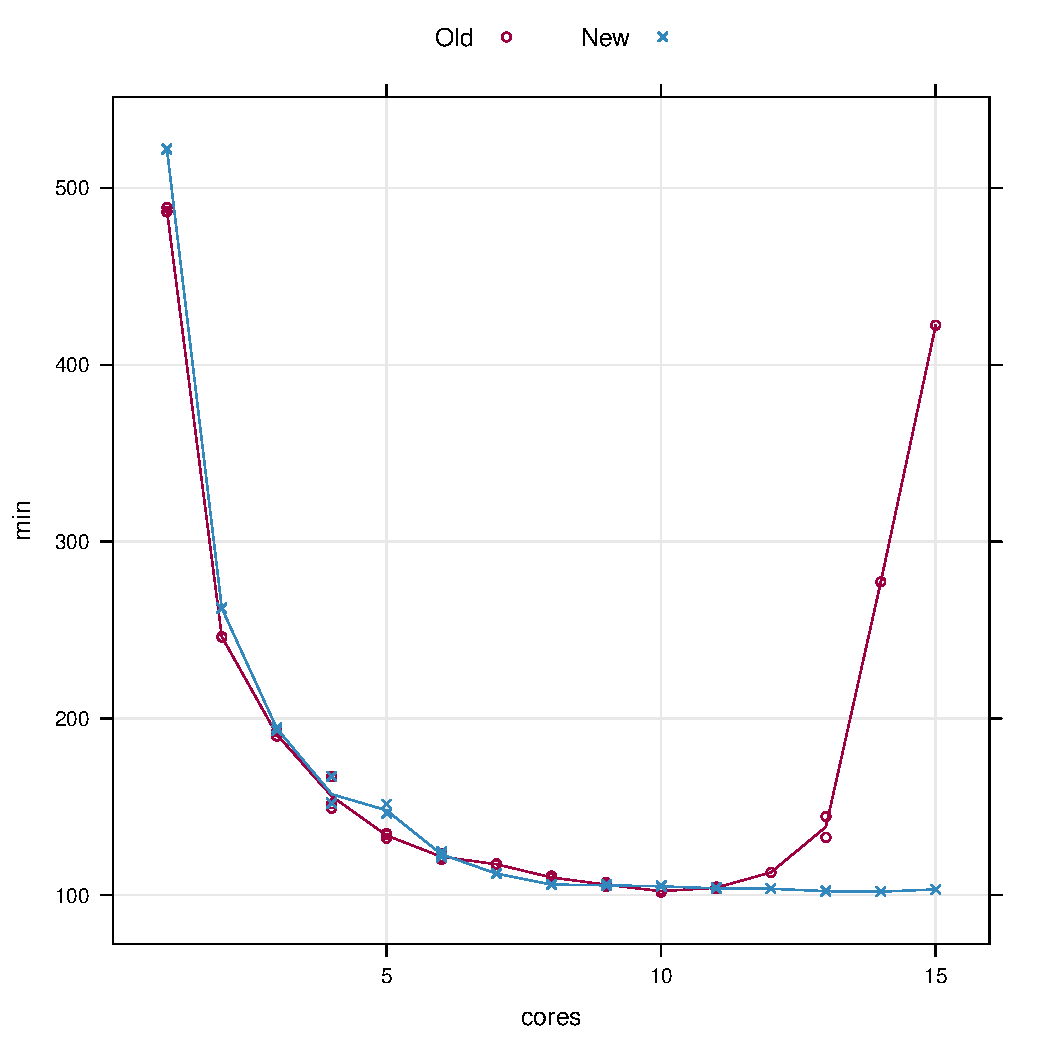
\includegraphics[clip, width = .4\textwidth]{min}    
    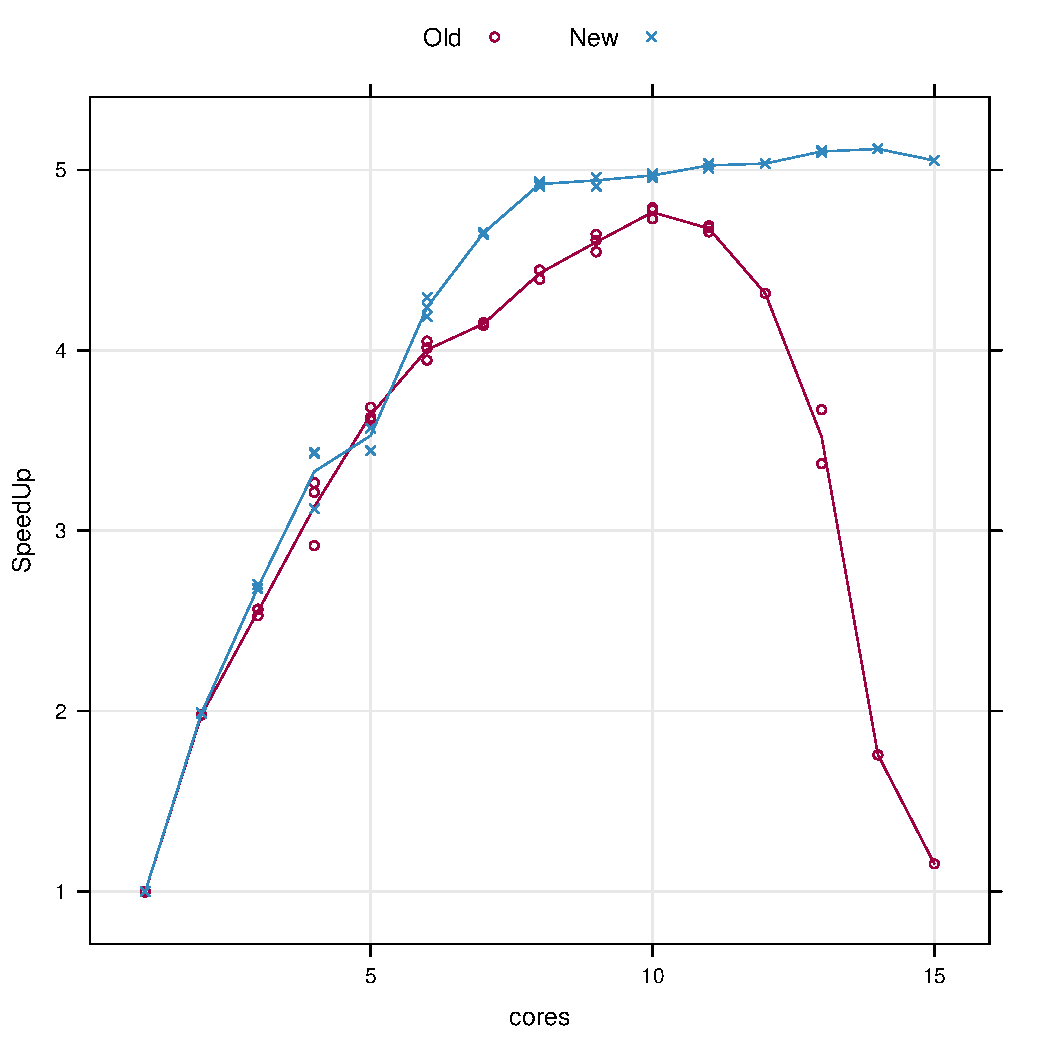
\includegraphics[clip, width = .4\textwidth]{speedup}
    \caption{Training time profiles using parallel processing via
      \pkg{caret} for a benchmarking data set run on a 16 core
      machine. The left panel shows the elapsed time to train
      a model using single or multiple
      processors. The panel on the right shows the ``speedup,''
      defined to be the time for serial execution divided by the
      parallel execution time. The ``old'' line corresponds to version
      4.98 and below while the ``new'' curve is using \pkg{foreach}.
    }
    \label{f:parallel}         
  \end{center}
\end{figure}

Figure \ref{f:parallel} shows the results of a benchmarking study run
on a 16 core machine. In the left panel, the actual training time for
a radial basis function SVM model for a data set with 5,000 samples
and 400 predictors. The model was tuned over 10 values of the cost
parameter using 50 bootstrap samples. The ``new'' curve corresponds to
the \pkg{foreach} infrastructure. 

One downside to parallel processing in this manner is that the dataset
is held in memory for every node used to train the model. For example,
if parallelism is used to compute the results from 50 bootstrap
samples using $P$ processors, $P$ data sets are held in memory. For
large datasets, this can become a problem if the additional processors
are on the same machines where they are competing for the same
physical memory. The old codebase starts to slow down around 10
workers due to exhausting the physical memory on the machine. The new
codebase does a better job at managing memory with no additional slowdown.


\section{Extracting Predictions and Class Probabilities}\label{S:probs}

As previously mentioned, objects produced by the \pkg{caret}
function contain the ``optimized'' model in the \code{finalModel}
sub--object. Predictions can be made from these objects as usual. In
some cases, such as \code{pls} or \code{gbm} objects, additional
parameters from the optimized fit may need to be specified. In these
cases, the \pkg{caret} objects uses the results of the parameter
optimization to predict new samples. 

For example, we can load the Boston Housing data:

\begin{small}
\begin{Schunk}
\begin{Sinput}
> library(mlbench)
> data(BostonHousing)
> # we could use the formula interface too
> bhDesignMatrix <-  model.matrix(medv ~. - 1, BostonHousing)
\end{Sinput}
\end{Schunk}
\end{small}

\noindent split the data into random training/test groups:

\begin{small}
\begin{Schunk}
\begin{Sinput}
> set.seed(4)
> inTrain <- createDataPartition(BostonHousing$medv, p = .8, list = FALSE, times = 1)
> trainBH <- bhDesignMatrix[inTrain,]
> testBH <- bhDesignMatrix[-inTrain,]
> trainMedv <- BostonHousing$medv[inTrain]
> testMedv <- BostonHousing$medv[-inTrain]
\end{Sinput}
\end{Schunk}
\end{small}

\noindent fit partial least squares and multivariate adaptive regression spline models:

\begin{small}
\begin{Schunk}
\begin{Sinput}
> set.seed(5)
> plsFit <- train(trainBH, trainMedv, 
+                 "pls", 
+                 preProcess = c("center", "scale"),
+                 tuneLength = 10, 
+                 trControl = trainControl(verboseIter = FALSE,
+                                          returnResamp = "all"))
> set.seed(5)
> marsFit <- train(trainBH, trainMedv, 
+                  "earth", 
+                  tuneLength = 10, 
+                  trControl = trainControl(verboseIter = FALSE,
+                                           returnResamp = "all"))
> 
\end{Sinput}
\end{Schunk}
\end{small} 
To obtain predictions  for the MARS model, \code{predict.earth} can be
used. 

\begin{small}
\begin{Schunk}
\begin{Sinput}
> marsPred1 <- predict(marsFit$finalModel, newdata = testBH)
> head(marsPred1)
\end{Sinput}
\begin{Soutput}
            y
[1,] 34.18241
[2,] 20.90113
[3,] 18.83659
[4,] 14.56850
[5,] 16.44564
[6,] 22.12989
\end{Soutput}
\end{Schunk}
\end{small}
Alternatively, \code{predict.train} can be used to get a vector of predictions for the optimal model only:
\begin{small}
\begin{Schunk}
\begin{Sinput}
> marsPred2 <- predict(marsFit, newdata = testBH)
> head(marsPred2)
\end{Sinput}
\begin{Soutput}
[1] 34.18241 20.90113 18.83659 14.56850 16.44564 22.12989
\end{Soutput}
\end{Schunk}
\end{small}
Note that the \code{plsFit} object used pre--processing. In this
case, we cannot directly call \code{predict.mvr} and expect to get
the same answers as \code{predict.train}. The latter function knows
that centering and scaling is required and execute these calculations
on the new samples, whereas \code{predict.mvr} does not. For the
\code{pls} function, there is an argument called \code{scale} that
can be used instead of the pre--processing options in the
\pkg{caret} function.

For multiple models, the objects can be grouped using a list and predicted simultaneously:
\begin{small}
\begin{Schunk}
\begin{Sinput}
> bhModels <- list(pls = plsFit, mars = marsFit)
> bhPred1 <- predict(bhModels, newdata = testBH)
> str(bhPred1)
\end{Sinput}
\begin{Soutput}
List of 2
 $ pls : num [1:99] 29 23.2 18 15 16 ...
 $ mars: num [1:99] 34.2 20.9 18.8 14.6 16.4 ...
\end{Soutput}
\end{Schunk}
\end{small}
In some cases,observed outcomes and their associated predictions may
be needed for a set of models. In this case,
\code{extractPrediction} can be used. This function takes a list of
models and test and/or unknown samples as inputs and returns a data
frame of predictions: 
\begin{small}
\begin{Schunk}
\begin{Sinput}
> allPred <- extractPrediction(bhModels,
+                              testX = testBH,
+                              testY = testMedv)
> testPred <- subset(allPred, dataType == "Test")
> head(testPred)
\end{Sinput}
\begin{Soutput}
     obs     pred model dataType object
408 34.7 28.97357   pls     Test    pls
409 21.7 23.24191   pls     Test    pls
410 20.2 17.95260   pls     Test    pls
411 15.2 15.01046   pls     Test    pls
412 15.6 16.03266   pls     Test    pls
413 14.5 18.40421   pls     Test    pls
\end{Soutput}
\begin{Sinput}
> ddply(testPred, .(model), defaultSummary)
\end{Sinput}
\begin{Soutput}
  model     RMSE  Rsquared
1 earth 4.605244 0.8016275
2   pls 6.169207 0.6449520
\end{Soutput}
\begin{Sinput}
> 
\end{Sinput}
\end{Schunk}
\end{small}
The output of \code{extractPrediction} is a data frame with columns:
   \begin{itemize}   
      \item \code{obs}, the observed data
      \item \code{pred}, the predicted values from each model
      \item \code{model}, a character string (``\code{rpart}'', ``\code{pls}'' etc.)
      \item \code{dataType}, a character string for the type of data:
      \begin{itemize}
         \item ``\code{Training}'' data are the predictions on the training data from
            the optimal model,
         \item ``\code{Test}'' denote the predictions on the test set (if one is specified),
         \item ``\code{Unknown}'' data are the predictions on the unknown samples (if specified). 
         Only the predictions are produced for these data. Also, if the quick prediction of the unknowns
         is the primary goal, the argument \code{unkOnly} can be used to only process the unknowns.
      \end{itemize}
   \end{itemize}      

Some classification models can produce probabilities for each
class. The functions \code{predict.train} and \code{predict.list}
can be used with the \code{type = "probs"} argument to produce data
frames of class probabilities (with one column per class). Also, the
function \code{extractProbs} can be used to get these probabilities
from one or more models. The results are very similar to what is
produced by \code{extractPrediction} but with columns for each
class. The column \code{pred} is still the predicted class from the
model.  


\section{Evaluating Test Sets}

A function, \code{postResample}, can be used obtain the same
performance measures as generated by \pkg{caret} for regression or
classification. 

\subsection{Confusion Matrices}\label{S:confusion}

\pkg{caret} also contains several functions that can be used to
describe the performance of classification models. The functions
\code{sensitivity}, \code{specificity}, \code{posPredValue} and
\code{negPredValue} can be used to characterize performance where
there are two classes. By default, the first level of the outcome
factor is used to define the ``positive'' result (i.e. the event of
interest), although this can be changed.  

The function \code{confusionMatrix} can also be used to summarize
the results of a classification model: 

\begin{small}
\begin{Schunk}
\begin{Sinput}
> mdrrPredictions <- extractPrediction(list(gbmFit3), testX = testDescr, testY = testMDRR)
> mdrrPredictions <- mdrrPredictions[mdrrPredictions$dataType == "Test",]
> sensitivity(mdrrPredictions$pred, mdrrPredictions$obs)
\end{Sinput}
\begin{Soutput}
[1] 0.8
\end{Soutput}
\begin{Sinput}
> confusionMatrix(mdrrPredictions$pred, mdrrPredictions$obs)
\end{Sinput}
\begin{Soutput}
Confusion Matrix and Statistics

          Reference
Prediction Active Inactive
  Active      120       30
  Inactive     30       84
                                          
               Accuracy : 0.7727          
                 95% CI : (0.7174, 0.8219)
    No Information Rate : 0.5682          
    P-Value [Acc > NIR] : 2.872e-12       
                                          
                  Kappa : 0.5368          
 Mcnemar's Test P-Value : 1               
                                          
            Sensitivity : 0.8000          
            Specificity : 0.7368          
         Pos Pred Value : 0.8000          
         Neg Pred Value : 0.7368          
             Prevalence : 0.5682          
         Detection Rate : 0.4545          
   Detection Prevalence : 0.5682          
                                          
       'Positive' Class : Active          
\end{Soutput}
\end{Schunk}
\end{small}

The ``no--information rate'' is the largest proportion of the observed
classes (there were more actives than inactives in this test set). A
hypothesis test is also computed to evaluate whether the overall
accuracy rate is greater than the rate of the largest class. Also, the
prevalence of the ``positive event'' is computed from the data (unless
passed in as an argument), the detection rate (the rate of true events
also predicted to be events) and the detection prevalence (the
prevalence of predicted events). 

Suppose a $2 \times 2$ table with notation

\begin{tabular}{r|c|c|}
                    & \multicolumn{2}{c}{{\bf Reference}}          \\
\cline{2-3}
         {\bf Predicted}  & Event     & No Event \\
\cline{2-3}
         Event      & A         & B        \\
\cline{2-3}
         No Event   & C         & D      \\
\cline{2-3}  
\end{tabular}

The formulas used here are:
\begin{align}
Sensitivity &= \frac{A}{A+C}\notag \\
Specificity &= \frac{D}{B+D}\notag \\
Prevalence &= \frac{A+C}{A+B+C+D}\notag \\
PPV &= \frac{sensitivity \times prevalence}{((sensitivity \times prevalence) + ((1-specificity) \times(1-prevalence))}\notag \\
NPV &= \frac{specificity \times (1-prevalence)}{((1-sensitivity) \times prevalence) + ((specificity) \times(1-prevalence))}\notag \\
Detection\: Rate &=  \frac{A}{A+B+C+D}\notag \\
Detection\: Prevalence &=  \frac{A + B}{A+B+C+D}\notag 
\end{align}

When there are three or more classes, \code{confusionMatrix} will
show the confusion matrix and a set of ``one--versus--all''
results. For example, in a three class problem, the sensitivity of the
first class is calculated against all the samples in the second and
third classes (and so on). 

Also, a resampled estimate of the training set can also be obtained
using \code{confusionMatrix.train}. For each resampling iteration,
a confusion matrix is created from the hold--out samples and these
values can be aggregated to diagnose issues with the model fit.

For example, in the two--class SVM model used in Section
\ref{S:basic}, we could use:

\begin{Schunk}
\begin{Sinput}
> confusionMatrix(gbmFit3)
\end{Sinput}
\begin{Soutput}
Cross-Validated (10 fold, repeated 3 times) Confusion Matrix 

(entries are percentages of table totals)
 
          Reference
Prediction Active Inactive
  Active     48.7     12.1
  Inactive    7.3     31.9
\end{Soutput}
\end{Schunk}

These values are the percentages that hold--out samples landed in the
confusion matrix during resampling. There are several methods for
normalizing these values. See \code{?confusionMatrix.train} for details.


\subsection{ROC Curves}\label{S:roc}

The function \code{roc}\footnote{I'm looking into using the
  \texttt{ROCR} package for ROC curves, so don't get too attached to
  these functions} can be used to calculate the sensitivity and
specificity used in an ROC plot. For example, using the previous
support vector machine fit to the MDRR data, the predicted class
probabilities on the test set can used to create an ROC curve. The
area under the ROC curve, via the trapezoidal rule, is calculated
using the \code{aucRoc} function.  

\begin{small}
\begin{Schunk}
\begin{Sinput}
> mdrrProbs <- extractProb(list(gbmFit3), testX = testDescr, testY = testMDRR)
> mdrrProbs <- mdrrProbs[mdrrProbs$dataType == "Test",]
> mdrrROC <- roc(mdrrProbs$Active, mdrrProbs$obs)
> aucRoc(mdrrROC)
\end{Sinput}
\begin{Soutput}
[1] 0.8726316
\end{Soutput}
\end{Schunk}
\end{small}

See Figure \ref{f:mdrrROC} for an example.

\subsection*{Plotting Predictions and Probabilities}

Two functions, \code{plotObsVsPred} and \code{plotClassProbs}, are
interfaces to lattice to plot model results. For regression,
\code{plotObsVsPred} plots the observed versus predicted values by
model type and data (e.g. test). See Figures \ref{f:bhPredPlot} and
\ref{f:mdrrROC}  for examples. For classification data,
\code{plotObsVsPred} plots the accuracy rates for models/data in a
dotplot.  



\begin{figure}
   \begin{center}      
      \includegraphics[clip, width = .5\textwidth]{gbmProbs}   
      \caption{The predicted class probabilities from a gradient boosting machine fit for the MDRR test set. This plot was created using \code{plotClassProbs(mdrrProbs)}.}
      \label{f:mdrrProbs}     
   \end{center}
\end{figure}  

\begin{figure}
   \begin{center}         
       \includegraphics[clip, width = .5\textwidth]{roc}   
      \caption{An ROC curve from the predicted class probabilities from a gradient boosting fit for the MDRR test set. }
      \label{f:mdrrROC}       
   \end{center}
\end{figure}  

\begin{figure}
   \begin{center}      
      \includegraphics[clip, width = .75\textwidth]{bhPredPlot}   
      \caption{The results of using \code{ plotObsVsPred } to show
        plots of the observed median home price against the
        predictions from two models. The plot shows the training and
        test sets in the same Lattice plot} 
      \label{f:bhPredPlot}         
   \end{center}
\end{figure}


To plot class probabilities, \code{plotClassProbs} will display the
results by model, data and true class (for example, Figure
\ref{f:mdrrProbs}).      

\clearpage

\section{Exploring and Comparing Resampling Distributions}

\subsection{Within--Model}\label{S:withinMod}

There are several Lattice functions than can be used to explore
relationships between tuning parameters and the resampling results for
a specific model:
\begin{itemize}
\item \code{xyplot} and \code{stripplot} can be used to plot resampling statistics
  against (numeric) tuning parameters.
  \item \code{histogram} and \code{densityplot} can also be used
      to look at distributions of the tuning parameters across tuning parameters.
\end{itemize}

For example, the following statements produces the images in Figure \ref{f:marsDesns}.   

\begin{small}
\begin{Schunk}
\begin{Sinput}
> xyplot(marsFit, type= c("g", "p", "smooth"), degree = 2)
> densityplot(marsFit, as.table = TRUE, subset = nprune < 10)
\end{Sinput}
\end{Schunk}
\end{small}



\begin{figure}[hb]
   \begin{center}      
      \includegraphics[clip, width = .7\textwidth]{marsXY}   
      
      \vspace{.3 in}      

       \includegraphics[clip, width = .7\textwidth]{marsDens}   
      \caption{Scatter plots and density plots of the resampled RMSE by the number of
        retained terms for the MARS model fit to the Boston Housing data}
      \label{f:marsDesns}       
   \end{center}
\end{figure}  
\clearpage

\subsection{Between--Models}\label{S:betweenMod}


\pkg{caret} also includes functions to characterize the differences
between models (generated using \pkg{caret}, \code{sbf} or
\code{rfe}) via their resampling distributions. These functions are
based on the work of Hothorn et al. (2005) and Eugster et al (2008).

Using the blood-brain barrier data (see \code{?BloodBrain)}, three regression models were
created: an \code{rpart} tree, a conditional inference tree using
\code{ctree}, M5 rules using \code{M5Rules} and a MARS model using
\code{earth}. We ensure that the models use the same resampling data
sets. In this case, 100 leave--group--out cross--validation was
employed. 

\begin{Schunk}
\begin{Sinput}
> data(BloodBrain)
> set.seed(1)
> tmp <- createDataPartition(logBBB, p = 0.8, times = 100)
> rpartFit <- train(bbbDescr, logBBB,
+                   "rpart", 
+                   tuneLength = 16,
+                   trControl = trainControl(method = "LGOCV", index = tmp, timingSamps = 50))
\end{Sinput}
\begin{Soutput}
Fitting: maxdepth=16 
\end{Soutput}
\begin{Sinput}
> ctreeFit <- train(bbbDescr, logBBB,
+                  "ctree2",
+                   tuneLength = 10,
+                   trControl = trainControl(method = "LGOCV", index = tmp, timingSamps = 50))
\end{Sinput}
\begin{Soutput}
Fitting: maxdepth=1 
Fitting: maxdepth=2 
Fitting: maxdepth=3 
Fitting: maxdepth=4 
Fitting: maxdepth=5 
Fitting: maxdepth=6 
Fitting: maxdepth=7 
Fitting: maxdepth=8 
Fitting: maxdepth=9 
Fitting: maxdepth=10 
\end{Soutput}
\begin{Sinput}
> earthFit <- train(bbbDescr, logBBB,
+                   "earth",
+                   tuneLength = 20,
+                   trControl = trainControl(method = "LGOCV", index = tmp, timingSamps = 50))
\end{Sinput}
\begin{Soutput}
Fitting: degree=1, nprune=76 
\end{Soutput}
\end{Schunk}
\begin{Sinput}
> m5Fit <- train(bbbDescr, logBBB,
+                "M5Rules",
+                trControl = trainControl(method = "LGOCV", index = tmp, timingSamps = 50))    
\end{Sinput}
\begin{Soutput}
Fitting: pruned=Yes 
Fitting: pruned=No 
\end{Soutput}


Given these models, can we make statistical statements about their
performance differences? To do this, we first collect the resampling
results using \code{resamples}. 

\begin{Schunk}
\begin{Sinput}
> resamps <- resamples(list(CART = rpartFit,
+                           CondInfTree = ctreeFit,
+                           MARS = earthFit,
+                           M5 = m5Fit))
> resamps
\end{Sinput}
\begin{Soutput}
Call:
resamples.default(x = list(CART = rpartFit, CondInfTree = ctreeFit,     MARS = earthFit, M5 = m5Fit))

Models: CART, CondInfTree, MARS, M5 
Number of resamples: 100 
Performance metrics: RMSE, Rsquared 
Time estimates for: everything, final model fit, prediction 
\end{Soutput}
\begin{Sinput}
> summary(resamps)
\end{Sinput}
\begin{Soutput}
Call:
summary.resamples(object = resamps)

Models: CART, CondInfTree, MARS, M5 
Number of resamples: 100 

RMSE 
              Min. 1st Qu. Median   Mean 3rd Qu.   Max.
CART        0.4927  0.5806 0.6417 0.6331  0.6764 0.7819
CondInfTree 0.4528  0.5934 0.6375 0.6427  0.6873 0.8685
MARS        0.4387  0.5709 0.6073 0.6128  0.6601 0.8327
M5          0.4607  0.5689 0.6219 0.6308  0.6763 0.8341

Rsquared 
               Min. 1st Qu. Median   Mean 3rd Qu.   Max.
CART        0.12070  0.2749 0.3436 0.3455  0.4049 0.5981
CondInfTree 0.07711  0.2852 0.3517 0.3449  0.4099 0.6164
MARS        0.18800  0.3381 0.4146 0.4141  0.4939 0.6515
M5          0.12260  0.3080 0.3910 0.3950  0.4744 0.6286
\end{Soutput}
\end{Schunk}

There are several Lattice plot methods that can be used to visualize
the resampling distributions: density plots, box--whisker plots,
scatterplot matrices and scatterplots of summary statistics. In the
latter case, the plot consists of a scatterplot between the two
models.  (See Figure
\ref{f:resampleScatter}). In Figure \ref{F:resampleDens}, density plots
of the data are shown. In this figure,  the $R^2$ distributions
indicate that M5 rules and MARS appear to be
similar to one another but different from the two tree--based
models. However, this pattern is inconsistent with the root
mean squared error distributions.

\begin{Schunk}
\begin{Sinput}
> bwplot(resamps, metric = "RMSE")
> densityplot(resamps, metric = "RMSE")
> xyplot(resamps,
+        models = c("CART", "MARS"),
+        metric = "RMSE")
> splom(resamps, metric = "RMSE")
\end{Sinput}
\end{Schunk}



Since models are fit on the same versions of the training data, it
makes sense to make inferences on the differences between models. In
this way we reduce the within--resample correlation that may exist. We
can compute the differences, then use a simple $t$--test to evaluate
the null hypothesis that there is no difference between models. 

\begin{Schunk}
\begin{Sinput}
> difValues <- diff(resamps)
> difValues
\end{Sinput}
\begin{Soutput}
Call:
diff.resamples(x = resamps)

Models: CART, CondInfTree, MARS, M5 
Metrics: RMSE, Rsquared 
Number of differences: 6 
p-value adjustment: bonferroni 
\end{Soutput}
\begin{Sinput}
> summary(difValues)
\end{Sinput}
\begin{Soutput}
Call:
summary.diff.resamples(object = difValues)

p-value adjustment: bonferroni 
Upper diagonal: estimates of the difference
Lower diagonal: p-value for H0: difference = 0

RMSE 
            CART      CondInfTree MARS      M5       
CART                  -0.009607    0.020238  0.002280
CondInfTree 0.8305096              0.029845  0.011887
MARS        0.0447524 0.0006745             -0.017958
M5          1.0000000 1.0000000   0.2662612          

Rsquared 
            CART      CondInfTree MARS       M5        
CART                   0.0005807  -0.0685809 -0.0495256
CondInfTree 1.000000              -0.0691617 -0.0501063
MARS        5.753e-08 6.541e-08               0.0190553
M5          0.002156  0.001024    0.679609             
\end{Soutput}
\end{Schunk}
Note that these results are consistent with the patterns shown in
Figure \ref{F:resampleDens}; there are more differences in the $R^2$
distributions than in the error distributions.

Several Lattices methods also exist to plot the differences (density
and box--whisker plots) or the inferential results (level and dot
plots). Figures \ref{F:diffLevel} and \ref{F:diffDot} show examples of
level and dot plots.

\begin{Schunk}
\begin{Sinput}
> dotplot(difValues)
> densityplot(difValues,
+             metric = "RMSE",
+             auto.key = TRUE,
+             pch = "|")
> bwplot(difValues,
+        metric = "RMSE")
> levelplot(difValues, what = "differences")
\end{Sinput}
\end{Schunk}



\begin{figure}
   \begin{center}		
      \includegraphics[clip, width = .6\textwidth]{resampleScatter}    

      \caption{ Examples of output from \code{xyplot(resamps, models = c("CART", "MARS"))}. }
      \label{f:resampleScatter} 
    \end{center}
\end{figure} 

\begin{figure}
   \begin{center}		
      \includegraphics[clip, width = .9\textwidth]{resampleDens}    

      \caption{ Examples of output from
        \code{densityplot(resamps)}. Looking at $R^2$, M5 rules and MARS appear to be
        similar to one another but different from the two tree--based
        models. However, this pattern is inconsistent with the root
        mean squared error distributions.}
      \label{F:resampleDens} 
    \end{center}
\end{figure} 


\begin{figure}
   \begin{center}		
      \includegraphics[clip, width = .8\textwidth]{diffLevel}    

      \caption{ Examples of output from \code{levelplot(difValues,
          what = "differences")}. The pair--wise differences in RMSE
        are shown}
      \label{F:diffLevel} 
    \end{center}
\end{figure} 


\begin{figure}
   \begin{center}		
      \includegraphics[clip, width = .8\textwidth]{diffDot}    

      \caption{ Examples of output from
        \code{dotplot(difValues)}. The differences in RMSE and their
        associated confidence intervals are shown.}
      \label{F:diffDot} 
    \end{center}
\end{figure} 


\section{Session Information}

\begin{itemize}\raggedright
  \item R version 2.13.1 Patched (2011-08-02 r56617), \verb|x86_64-apple-darwin9.8.0|
  \item Locale: \verb|en_US.UTF-8/en_US.UTF-8/C/C/en_US.UTF-8/en_US.UTF-8|
  \item Base packages: base, datasets, graphics, grDevices, grid,
    methods, splines, stats, stats4, utils
  \item Other packages: caret~4.99, class~7.3-3, cluster~1.14.0,
    codetools~0.2-8, doMC~1.2.2, e1071~1.5-26, earth~3.2-1,
    foreach~1.3.2, gbm~1.6-3.1, ipred~0.8-11, iterators~1.0.5,
    kernlab~0.9-12, lattice~0.19-31, leaps~2.9, MASS~7.3-14,
    mlbench~2.1-0, modeltools~0.2-17, multicore~0.1-5,
    mvtnorm~0.9-9991, nnet~7.3-1, plotmo~1.2-6, plotrix~3.2-2,
    pls~2.1-0, plyr~1.5.2, randomForest~4.6-2, reshape~0.8.4,
    rpart~3.1-50, survival~2.36-9
  \item Loaded via a namespace (and not attached): coin~1.0-18,
    colorspace~1.1-0, compiler~2.13.1, party~0.9-99992, rJava~0.9-1,
    RWeka~0.4-7, RWekajars~3.7.3-1, tools~2.13.1
\end{itemize}

\section{References}

\begin{description}

  
\item Breiman, Friedman, Olshen, and Stone. (1984) {\it Classification
    and Regression Trees}. Wadsworth. 

\item Eugster et al. (2008),  ``Exploratory and inferential analysis
  of benchmark experiments, '' {\it Ludwigs-Maximilians-Universitat
    Munchen, Department of Statistics, Tech. Rep} vol. 30 
  
  
\item Hothorn et al. (2005),  ``The design and analysis of
  benchmark experiments, '' {\it Journal of Computational and
    Graphical Statistics}, 14,  675--699

  \item Molinaro et al. (2010), ``partDSA:
    deletion/substitution/addition algorithm for partitioning the
    covariate space in prediction,'' {\it Bioinformatics}, 26, 1357--1363

\item Rand (1971),  ``Objective criteria for the evaluation of
  clustering methods,'' {\it Journal of the American Statistical
    Association} 66, 846--850. 
    
\item Schmidberger et al. (2009), `` State-of-the-art in Parallel
  Computing with R,'' {\it Journal of Statistical Software}, 31
  
\item Svetnik, V., Wang, T., Tong, C., Liaw, A., Sheridan, R. P. and
  Song, Q. (2005), ``Boosting: An ensemble learning tool for compound
  classification and QSAR modeling,'' {\it Journal of Chemical
    Information and Modeling}, 45, 786 --799. 
  
\item Tibshirani, R., Hastie, T., Narasimhan, B., Chu, G. (2003),
  ``Class prediction by nearest shrunken centroids, with applications
  to DNA microarrays,'' {\it  Statistical Science}, 18, 104--117. 

\end{description}

\end{document}
